% !TeX root = ../main.tex
\section{Design}
\label{sec:overview}
\label{sec:method}
Figure~\ref{fig:overview} separates offline plan construction from online expert delivery.
The expert planner receives layer/expert counts, skew parameters, model metadata, and primary residency budgets.
It allocates capacities and ranks expert IDs within each layer.
The loader initializes HBM and CPU from this plan.
HDD retains the full expert pool and supplies weights absent from both resident tiers.

Consider the selected experts $e_2$ and $e_6$ in the framework.
The lookup finds $e_2$ in CPU memory and $e_6$ on HDD.
Promoting $e_2$ creates an HBM resident and frees its CPU slot.
The runtime uses that slot to retain the expert displaced from HBM.
Reading $e_6$ then supplies another requested expert through the HDD--CPU--GPU path.
Each expert executes after its transfer completes.
The model combines their outputs with the gate weights and continues to the next layer.

The cache state persists across tokens and requests.
Each routed access updates expert recency within the layer's allocated capacities.
An expert request carries both a layer index and a local expert ID.
The same local ID in another layer refers to a different weight block.
Advancing through the model preserves the earlier layers' residents.
Offline planning determines the starting state; routed accesses determine its subsequent membership.

\subsection{Expert Planner}
\label{sec:expert_planner}
\begin{figure}[H]
\centering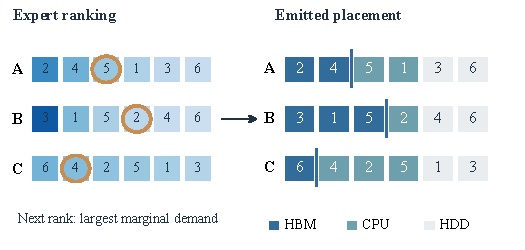
\includegraphics[width=\columnwidth]{figures/fig04_compile_frontiers.pdf}
\par\nointerlineskip
\caption{Planning the initial state.
The left grid contains ranked per-layer demand; circles mark the next uncovered candidates.
Shared HBM/CPU slot budgets produce different cuts in the emitted rows.
A, B, and C identify different layers.
}
\label{fig:compile}
\end{figure}

Consider $L$ MoE layers with $N_\ell$ experts per layer.
For the routed pools considered here, experts have equal size $s$ and layers use the same top-$k$.

Primary expert-residency budgets $B_{\mathrm H}$ and $B_{\mathrm C}$ provide $S_{\mathrm H}=\lfloor B_{\mathrm H}/s\rfloor$ HBM slots and $S_{\mathrm C}=\lfloor B_{\mathrm C}/s\rfloor$ CPU slots.
Physical host usage includes CPU residents, GPU-weight mirrors, and staging buffers.

Calibration orders experts by selection counts.
The analysis collects selected expert IDs separately for each layer.
Let $\pi_\ell(r)$ denote the local ID at rank $r$ in layer $\ell$.
Expert ID breaks equal-count ties.
Zero-count IDs follow observed experts in ID order.
The planner therefore compares demand across layers while preserving a separate expert list for each layer.
A log-count versus log-rank regression supplies $\alpha_\ell$ as the negative slope over positive counts.
The rank model smooths the observed selection frequencies for allocation scoring:
\begin{equation}
q_{\ell,r}=\frac{r^{-\alpha_\ell}}{\sum_{j=1}^{N_\ell}j^{-\alpha_\ell}}.
\end{equation}
Here $q_{\ell,r}$ is conditional selection mass within layer $\ell$, with unit sum.
Equal top-$k$ makes this mass comparable across layers.
Counts determine which expert occupies each rank; the rank model supplies the allocation scores.

Figure~\ref{fig:compile} shows the HBM and CPU cuts in those lists.
Capacities satisfy $\sum_\ell K_{\mathrm H,\ell}\le S_{\mathrm H}$, $\sum_\ell K_{\mathrm C,\ell}\le S_{\mathrm C}$, and $K_{\mathrm H,\ell}+K_{\mathrm C,\ell}\le N_\ell$.
The adaptive scan reserves one slot per layer in each fast tier, then distributes the remaining slots by marginal coverage.
The reservation accounts for $L$ slots in each tier before the remaining allowance is distributed.

The scan first assigns HBM slots.
At each step, it chooses the layer with the largest next-rank score:
\begin{equation}
\Delta_\ell=q_{\ell,K_{\mathrm H,\ell}+1}.
\end{equation}
CPU allocation continues from the first ranks beyond each HBM cut.
Its next candidate has score
\begin{equation}
\Delta^{\mathrm C}_\ell=q_{\ell,K_{\mathrm H,\ell}+K_{\mathrm C,\ell}+1}.
\label{eq:cpu_marginal}
\end{equation}
The HBM offset directs CPU slots to experts beyond those already selected for the GPU.
An eligible layer has an uncovered expert within its local list.
The scan compares these candidates, assigns one slot, and advances the selected layer's cut.
Every allocation exposes a new next-rank candidate in that layer.
Layer ID breaks score ties, and expert ID breaks count ties.
The direct scan takes $O(L(S_{\mathrm H}+S_{\mathrm C}))$ time after sorting.
Its score is the additional within-layer selection mass covered by the next slot.
Sorting the layer-local lists takes $O(\sum_\ell N_\ell\log N_\ell)$ time.

The expert planner serializes a residency plan: model dimensions, expert size, capacity arrays, and ranked layer-local IDs.
For layer $\ell$, ranks $1$ through $K_{\mathrm H,\ell}$ enter HBM.
Ranks $K_{\mathrm H,\ell}+1$ through $K_{\mathrm H,\ell}+K_{\mathrm C,\ell}$ enter the CPU resident set.
All other ranks remain available from the backing store.
The JSON plan is the deployment artifact consumed by the loader.
The loader constructs a cache for each layer from the corresponding IDs and capacities.
The capacity arrays remain fixed during serving.
Changing task demand updates the residents through online admission.

\subsection{Expert Retention}
\label{sec:expert_retention}
Each layer maintains two ordered sets, from most-recently used (MRU) to least-recently used (LRU).
Their concatenation places HBM residents before CPU residents.
The two primary sets contain distinct expert IDs.
The ordering describes recency across both managed tiers.
An HBM hit moves its expert to HBM MRU.
A CPU hit removes its host entry and promotes it to HBM MRU.
The evicted GPU LRU expert then becomes CPU MRU.
HDD retains the backing weights for every expert.
The cold payload comes from a completed read or a pending read resolved at consumption.
It enters HBM MRU and follows the same demotion rule as a CPU promotion.
If this admission exceeds the CPU capacity, the CPU LRU entry is removed.
The backing store supplies that expert again when a later request misses both tiers.

\begin{figure}[H]
\centering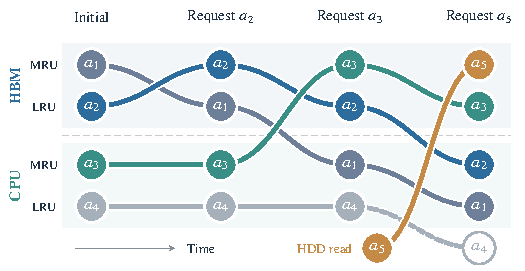
\includegraphics[width=\columnwidth]{figures/fig05_residency_cases.pdf}
\par\nointerlineskip
\caption{Expert recency over three requests.
Colored tracks follow the same experts from left to right.
Within each tier, the upper position is MRU and the lower position is LRU.
A CPU hit promotes $a_3$ and retains $a_1$ on the host.
Loading $a_5$ from HDD retains $a_2$ and removes $a_4$ from CPU.}
\label{fig:retention}
\end{figure}
Figure~\ref{fig:retention} starts with HBM $[a_1,a_2]$ and CPU $[a_3,a_4]$.
Request $a_2$ gives HBM $[a_2,a_1]$.
Request $a_3$ then promotes $a_3$ and demotes $a_1$, producing HBM $[a_3,a_2]$ and CPU $[a_1,a_4]$.
Finally, $a_5$ enters HBM, $a_2$ becomes CPU MRU, and $a_4$ leaves CPU LRU.
The final lists are $[a_5,a_3]$ and $[a_2,a_1]$.

Each GPU resident carries a host mirror.
The implementation stores device weights and their host tensor together in the GPU entry.
On promotion, the CPU resident's host tensor continues as the promoted expert's mirror.
The released slot is a logical CPU residency entry.
The demoted expert's existing mirror becomes the new resident named by that entry.
This exchange retains the demoted weights through a metadata update and saves a device-to-host copy.

Mirrors and CPU residents serve different roles.
A mirror supports an expert currently assigned to HBM; a CPU resident supplies an expert outside the HBM set.
For equal-size blocks and full resident sets, their steady host payload is $s\sum_\ell(K_{\mathrm H,\ell}+K_{\mathrm C,\ell})$.
Pending reads and staging buffers add to this payload.
Deployment sizing includes these allocations alongside the primary CPU capacity.

The ordered maps support lookup and recency updates in expected constant time.
A CPU hit consumes one CPU entry before admitting the requested expert to HBM.
A cold access introduces a new resident and may remove the CPU tail.
After each access, the primary sets respect their assigned capacities.
Active tensor references extend the lifetime of weights through expert execution.

\subsection{Online Execution}
\label{sec:weight_delivery}
Serving requests update the initial state through the same access rules.
When a task selects different experts, its first accesses admit them to HBM.
Subsequent demotions place them at CPU MRU, while older CPU entries move toward replacement.
HBM hits refresh recency directly.
The updated state survives the end of a prompt and serves later requests on the same model instance.

For each MoE layer, the wrapper evaluates the gate and groups token rows by selected expert.
The loader resolves each layer-local expert ID through the memory tiers.
The expert kernel processes its assigned rows.
Gate weights scale the outputs before accumulation into the layer result.
The gate continues to determine expert selection and mixture weights.

During prefill, the loader submits reads for the selected experts absent from memory.
Each read is resolved when its expert reaches consumption.
Figure~\ref{fig:delivery} shows resident work overlapping a pending read for another selected expert.

\begin{figure}[H]
\centering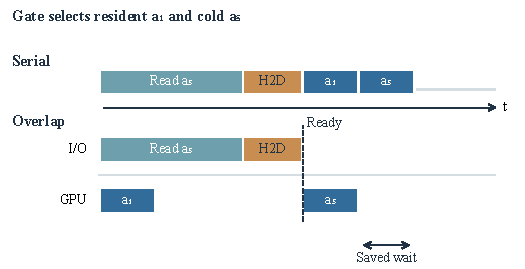
\includegraphics[width=\columnwidth]{figures/fig06_delivery_overlap.pdf}
\par\nointerlineskip
\caption{Prefill delivery for resident $a_1$ and cold $a_5$.
Computing $a_1$ overlaps the pending read for $a_5$.
H2D completion releases $a_5$ for GPU execution; the shortened schedule saves exposed waiting time.
}
\label{fig:delivery}
\end{figure}
A read future returns the host tensors that supply H2D.
The copy stream moves them to the GPU.
The loader synchronizes pending copies before yielding device tensors to computation.
The expert kernel then consumes those tensors.
Recording the consumer stream keeps their storage live through kernel completion.
These dependencies connect read completion, copy completion, and expert execution.

Prefill can request more experts than a single resident set holds.
The loader batches CPU-resident experts when the group fits the configured HBM slot count.
Larger groups use sequential access and eviction.
Temporary transfer buffers and active references form part of runtime memory use alongside managed residents.
Token generation uses the selected experts available for the current step.
An HBM hit executes with existing device weights; other accesses take the corresponding host or HDD delivery path.

Prefetchers use access analysis or lookahead to anticipate expert demand~\cite{pregated,fate,expertflow}.
Batch and request schedulers expose work from concurrent inputs~\cite{klotski,bevy}; distributed edge schemes add network delivery~\cite{odmoe}.
MECC combines request-driven retention with delivery of the experts selected at the current gate.
Retention determines which weight blocks remain available across accesses.
Delivery schedules the reads and copies that those accesses require.
Recency updates change metadata and resident references. Reads and copies provide a new physical placement when the selected expert requires one.
